\documentclass[aspectratio=169,11pt]{beamer}

\usepackage[utf8]{inputenc}
\usepackage[T1]{fontenc}
\usepackage[scaled=0.94]{helvet}
\renewcommand{\familydefault}{\sfdefault}
\usepackage[expansion=false]{microtype}
\usepackage{amsmath}
\usepackage{booktabs}
\usepackage{graphicx}
\usepackage{tikz}
\usetikzlibrary{arrows.meta,positioning,shapes.geometric,calc}

\graphicspath{%
  {../../services/inference/data/figures/}%
  {../../services/inference/data/final/report/}%
  {../../services/inference/data/paper1/}%
  {../thesis/assets/}%
}

% Three colours only: primary, accent, alert.
\definecolor{navy}{HTML}{1F4E79}
\definecolor{midblue}{HTML}{2E75B6}
\definecolor{ember}{HTML}{C0392B}
\definecolor{slate}{HTML}{595959}
\definecolor{mist}{HTML}{D9D9D9}

\usetheme{default}
\newcommand{\display}{\raggedright\hyphenpenalty=10000\exhyphenpenalty=10000\relax}
\setbeamercolor{background canvas}{bg=white}
\setbeamercolor{normal text}{fg=black}
\setbeamercolor{frametitle}{fg=navy}
\setbeamercolor{structure}{fg=navy}
\setbeamercolor{alerted text}{fg=ember}
\setbeamerfont{frametitle}{series=\bfseries,size=\large}
\setbeamertemplate{navigation symbols}{}
\setbeamertemplate{itemize items}{\color{navy}\textbf{\textbullet}}

\newlength{\slidemargin}
\setlength{\slidemargin}{1.15cm}
\setbeamersize{text margin left=\slidemargin,text margin right=\slidemargin}

% Action title, set on white with whitespace under it rather than a rule.
\setbeamertemplate{frametitle}{%
  \vspace{0.75em}%
  \begin{minipage}{\dimexpr\paperwidth-2\slidemargin\relax}
    \raggedright\usebeamerfont{frametitle}\usebeamercolor[fg]{frametitle}\insertframetitle%
  \end{minipage}%
  \vspace{0.35em}%
}

\setbeamertemplate{footline}{%
  \hspace{\slidemargin}%
  {\color{slate}\scriptsize\insertsection}%
  \hfill
  {\color{slate}\scriptsize\insertframenumber}%
  \hspace{\slidemargin}\vspace{0.8em}%
}

\newcommand{\naa}{\mathrm{NAA}}

% Source line, bottom of slide, muted.
\newcommand{\source}[1]{\par\vspace{0.5em}{\color{slate}\scriptsize #1}}

% One number, one line about it.
\newcommand{\heroslide}[3]{%
  \begin{frame}[plain]
    \vfill
    \begin{center}
      {\color{slate}\small\MakeUppercase{#1}}\\[0.9em]
      {\color{navy}\fontsize{50}{50}\selectfont\bfseries #2}\\[1.1em]
      \begin{minipage}{0.78\textwidth}\centering\large #3\end{minipage}
    \end{center}
    \vfill
  \end{frame}%
}

\newcommand{\act}[3]{%
  \begin{frame}[plain]
    \vfill
    \hspace{0.10\textwidth}%
    \begin{minipage}{0.8\textwidth}
      \display
      {\color{midblue}\fontsize{38}{38}\selectfont\bfseries #1}\\[0.5em]
      {\color{navy}\fontsize{25}{29}\selectfont\bfseries #2}\\[0.7em]
      {\color{slate}\large #3}
    \end{minipage}
    \vfill
  \end{frame}%
}

\title{Measuring the External Field}
\author{Brian Mwai}
\date{September 2026}

\begin{document}

% ================================================================ TITLE
\begin{frame}[plain]
\vfill
\hspace{0.08\textwidth}%
\begin{minipage}{0.84\textwidth}
\display
{\color{slate}\small B.Sc.\ PHYSICS \quad$\cdot$\quad DEPARTMENT OF NATURAL SCIENCES \quad$\cdot$\quad CUEA}

\vspace{1.2em}
{\color{navy}\fontsize{34}{40}\selectfont\bfseries Measuring the External Field}

\vspace{0.7em}
{\color{slate}\fontsize{15}{21}\selectfont A cortical-proxy content observable and the
mean-field bound on media-driven opinion change}

\vspace{1.5em}
{\color{mist}\hrule height 1.2pt}
\vspace{1.0em}

{\large\bfseries Brian Mwai} \quad{\color{slate} 1050555}\hfill
{\color{slate} Supervisor: Dr.\ Songa Mutambi}

\vspace{0.4em}
{\color{slate}\small September 2026}
\end{minipage}
\vfill
\end{frame}

% ================================================================ THE CLAIM, FIRST
\begin{frame}[plain]
\vfill
\hspace{0.10\textwidth}%
\begin{minipage}{0.80\textwidth}
\display
{\fontsize{15}{22}\selectfont
Statistical physics has always modelled media as a \textbf{field} pushing on a population of
coupled opinions.

\vspace{0.45em}
That field is assumed. It is not measured.\par}

\vspace{1.0em}
{\color{mist}\hrule height 1.2pt}
\vspace{1.0em}

{\fontsize{15}{22}\selectfont\color{navy}\bfseries
This project measures one from content itself, applies it to 400 articles, and derives how
strong the coupling would have to be for a spread that size to move a population at all.\par}
\end{minipage}
\vfill
\end{frame}

% ================================================================ ACT I
\section{The problem}
\act{01}{The problem}{What is missing from the way media is modelled.}

\begin{frame}{Two articles can report one event and leave readers in different states}
\vspace{0.3em}
\begin{center}
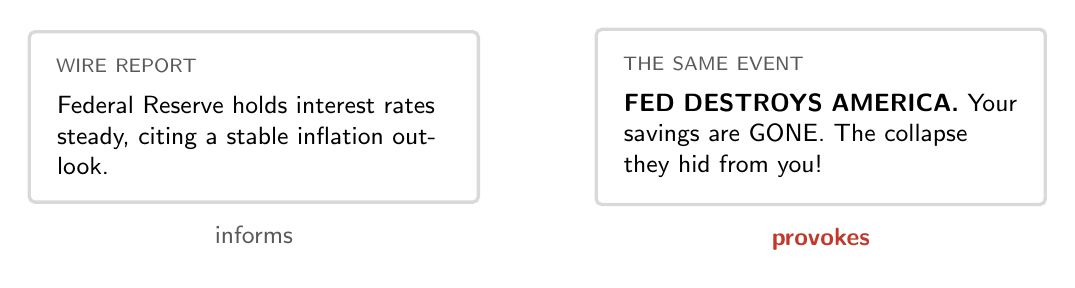
\begin{tikzpicture}[font=\small]
  \node[draw=mist,line width=1.2pt,rounded corners=2pt,fill=white,
        text width=5.0cm,inner sep=10pt,align=left] (a) at (0,0)
       {{\color{slate}\scriptsize WIRE REPORT}\\[0.4em]
        Federal Reserve holds interest rates steady, citing a stable inflation outlook.};
  \node[draw=mist,line width=1.2pt,rounded corners=2pt,fill=white,
        text width=5.0cm,inner sep=10pt,align=left] (b) at (7.2,0)
       {{\color{slate}\scriptsize THE SAME EVENT}\\[0.4em]
        \textbf{FED DESTROYS AMERICA.} Your savings are GONE. The collapse they hid from
        you!};
  \node[below=0.45em of a,text width=5.0cm,align=center,slate] {informs};
  \node[below=0.45em of b,text width=5.0cm,align=center,ember] {\textbf{provokes}};
\end{tikzpicture}
\end{center}

\vspace{0.9em}
Readers notice the difference and cannot quantify it. The platforms distributing both have no
objective measure of which they are amplifying.
\end{frame}

\begin{frame}{Existing tools measure the words; none measures the predicted response}
\vspace{0.9em}
\begin{center}
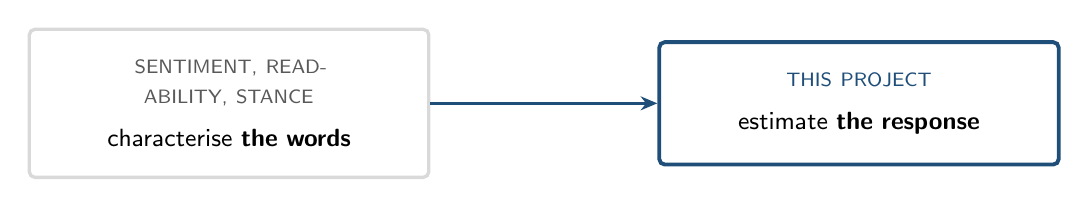
\begin{tikzpicture}[font=\small]
  \node[text width=4.3cm,align=center,draw=mist,line width=1.2pt,rounded corners=2pt,
        fill=white,inner sep=11pt] (old) at (0,0)
       {{\color{slate}\scriptsize SENTIMENT, READABILITY, STANCE}\\[0.5em]
        characterise \textbf{the words}};
  \node[text width=4.3cm,align=center,draw=navy,line width=1.4pt,rounded corners=2pt,
        fill=white,inner sep=11pt] (new) at (8.0,0)
       {{\color{navy}\scriptsize THIS PROJECT}\\[0.5em] estimate \textbf{the response}};
  \draw[-{Stealth[length=6pt,width=5pt]},line width=1.2pt,navy] (old) -- (new);
\end{tikzpicture}
\end{center}

\vspace{1.2em}
A released neural encoder predicts cortical activity from the content, and the measurement is
taken on that prediction.

\vspace{0.6em}
{\color{slate} The instrument is a thermometer for one property of media. The thesis is an
account of building it, running it, and stating what its readings support.}
\end{frame}

% ================================================================ ACT II
\section{The instrument}
\act{02}{The instrument}{From a passage of text to a single number.}

\begin{frame}{A five-stage cascade turns one article into one number}
\vspace{0.9em}
\begin{center}
\resizebox{\textwidth}{!}{%
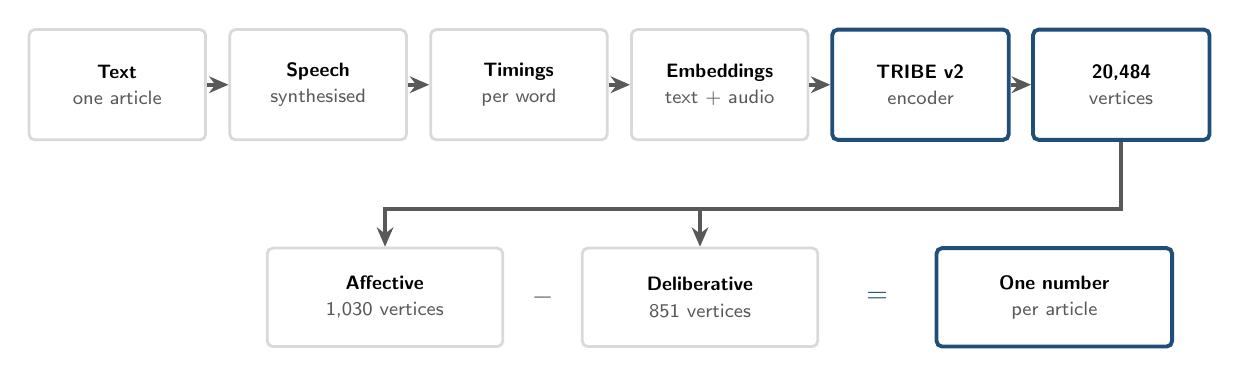
\begin{tikzpicture}[font=\scriptsize,
    box/.style={draw=mist,line width=1pt,rounded corners=2pt,fill=white,
                text width=1.75cm,align=center,inner sep=7pt,minimum height=1.4cm},
    hot/.style={draw=navy,line width=1.4pt,rounded corners=2pt,fill=white,
                text width=1.75cm,align=center,inner sep=7pt,minimum height=1.4cm},
    flow/.style={-{Stealth[length=7pt,width=6pt]},line width=1.3pt,slate}]
  \node[box] (t)  at (0,0)    {\textbf{Text}\\[0.2em]{\color{slate}one article}};
  \node[box] (s)  at (2.55,0) {\textbf{Speech}\\[0.2em]{\color{slate}synthesised}};
  \node[box] (w)  at (5.10,0) {\textbf{Timings}\\[0.2em]{\color{slate}per word}};
  \node[box] (e)  at (7.65,0) {\textbf{Embeddings}\\[0.2em]{\color{slate}text + audio}};
  \node[hot] (m)  at (10.20,0){\textbf{TRIBE v2}\\[0.2em]{\color{slate}encoder}};
  \node[hot] (v)  at (12.75,0){\textbf{20,484}\\[0.2em]{\color{slate}vertices}};
  \foreach \a/\b in {t/s,s/w,w/e,e/m,m/v} \draw[flow] (\a) -- (\b);

  \node[box,text width=2.5cm,minimum height=1.25cm] (aff) at (3.4,-2.7)
       {\textbf{Affective}\\[0.2em]{\color{slate}1,030 vertices}};
  \node[box,text width=2.5cm,minimum height=1.25cm] (del) at (7.4,-2.7)
       {\textbf{Deliberative}\\[0.2em]{\color{slate}851 vertices}};
  \node[hot,text width=2.5cm,minimum height=1.25cm] (out) at (11.9,-2.7)
       {\textbf{One number}\\[0.2em]{\color{slate}per article}};

  \draw[flow] (v.south) -- ++(0,-0.85) -| (aff.north);
  \draw[flow] (v.south) ++(0,-0.85) -| (del.north);
  \node[slate,font=\normalsize] at (5.4,-2.7) {$-$};
  \node[navy,font=\normalsize] at (9.65,-2.7) {$=$};
\end{tikzpicture}}
\end{center}
\source{Encoder: TRIBE v2, d'Ascoli et al., Meta FAIR (2025), arXiv:2507.22229. Regions from
HCP MMP1.0, Glasser et al.\ (2016). Instrument at \texttt{monarch-4iy.pages.dev}.}
\end{frame}

\begin{frame}{The index contrasts two cortical networks, 1,030 vertices against 851}
\vspace{-0.4em}
\begin{center}
\includegraphics[width=0.88\textwidth,trim=0 0 0 22,clip]{B1_roi_definition.pdf}
\end{center}
\vspace{-0.7em}
\begin{center}
{\color{slate}\small Affective salience in orange, deliberative control in blue. Resolved once
into vertex index sets and cached, so all 400 items are averaged over identical regions.}
\end{center}
\source{Regions defined on HCP MMP1.0 (Glasser et al., 2016); surfaces are fsaverage5.}
\end{frame}

\begin{frame}{The observable is a signed difference, defined for every item}
\vspace{1.2em}
\begin{center}
{\fontsize{26}{30}\selectfont\color{navy}
$\naa_{\text{signed}} \;=\; A_{\text{aff}} - A_{\text{del}}$}
\end{center}

\vspace{1.4em}
\begin{center}
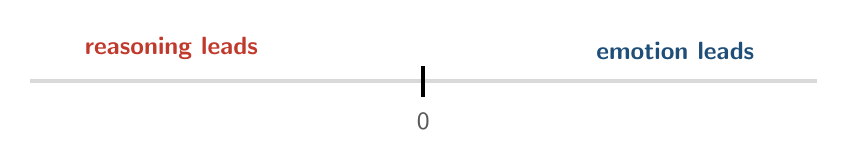
\begin{tikzpicture}[font=\small]
  \draw[line width=1.4pt,mist] (-5.0,0) -- (5.0,0);
  \draw[line width=1.4pt,black] (0,-0.2) -- (0,0.2);
  \node[below=0.3em] at (0,-0.18) {\color{slate}0};
  \node[above=0.45em,ember] at (-3.2,0) {\textbf{reasoning leads}};
  \node[above=0.45em,navy] at (3.2,0) {\textbf{emotion leads}};
\end{tikzpicture}
\end{center}

\vspace{1.3em}
A \textbf{cortical proxy}: it rates content, never a person, and is never called the amygdala.
\end{frame}

\begin{frame}{Inspecting the checkpoint changed what the project could claim}
\vspace{0.5em}
\begin{columns}[T]
\begin{column}{0.315\textwidth}
{\color{midblue}\bfseries\large 01}\\[0.3em]
\textbf{Cortical only}\\[0.4em]
{\small No subcortical output.

\vspace{0.5em}
\alert{No amygdala}, so the proposal's equation cannot be computed.}
\end{column}
\begin{column}{0.315\textwidth}
{\color{midblue}\bfseries\large 02}\\[0.3em]
\textbf{Averaged over subjects}\\[0.4em]
{\small The loader forces it.

\vspace{0.5em}
It predicts a typical viewer, which Paper 3 tests.}
\end{column}
\begin{column}{0.315\textwidth}
{\color{midblue}\bfseries\large 03}\\[0.3em]
\textbf{Standardised output}\\[0.4em]
{\small Means sit near zero, so a \emph{ratio} breaks.

\vspace{0.5em}
Undefined for 69 of 400 items; the difference replaces it.}
\end{column}
\end{columns}

\vspace{1.0em}
{\color{slate} All three were found by testing the checkpoint, before any result.}
\end{frame}

% ================================================================ ACT III
\section{The measurement}
\act{03}{The measurement}{400 articles, scanned twice.}

\begin{frame}{The corpus is length-matched and was powered before the scan}
\vspace{0.4em}
\begin{center}
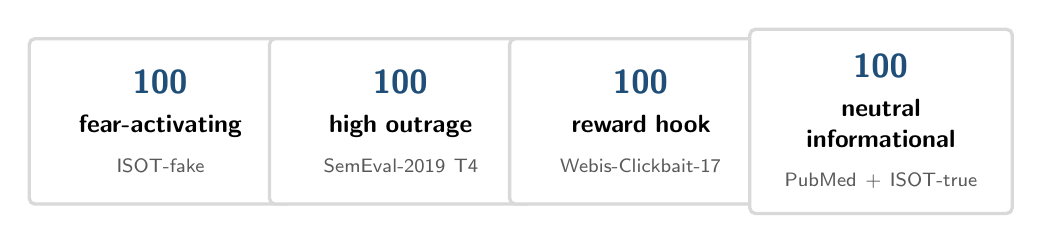
\begin{tikzpicture}[font=\small]
  \foreach \i/\name/\src in {%
    0/{fear-activating}/{ISOT-fake},
    1/{high outrage}/{SemEval-2019 T4},
    2/{reward hook}/{Webis-Clickbait-17},
    3/{neutral\\informational}/{PubMed + ISOT-true}}
  {
    \node[draw=mist,line width=1.2pt,rounded corners=2pt,fill=white,
          text width=2.7cm,align=center,inner sep=9pt,minimum height=2.1cm]
          at ({\i*3.05},0)
         {{\color{navy}\bfseries\large 100}\\[0.35em]\textbf{\name}\\[0.35em]
          {\color{slate}\scriptsize \src}};
  }
\end{tikzpicture}
\end{center}

\vspace{1.0em}
\textbf{Length-matched.} Mean word counts 167.4, 163.5, 163.7, 162.2; standard deviations
near 11.

\vspace{0.4em}
\textbf{Powered first.} Smallest detectable $\eta^2 = 0.0268$, smallest detectable AUC
$= 0.5916$, both fixed before a single item was scanned.

\source{Corpora: Ahmed et al.\ (ISOT, 2017); Kiesel et al.\ (SemEval-2019 Task 4);
Potthast et al.\ (Webis-Clickbait-17); PubMed open abstracts.}
\end{frame}

\heroslide{the four categories separate at}{$\eta^{2} = 0.1068$}%
{$F = 15.779$, \; $p = 1.03\times10^{-9}$, \; $n = 400$ \\[0.5em]
{\color{slate} against a design powered to detect $0.0268$}}

\begin{frame}{Categories shift against each other, but the distributions overlap}
\vspace{-0.2em}
\begin{center}

\includegraphics[width=0.76\textwidth]{fig_violin.png}
\end{center}
\vspace{-0.5em}
\begin{center}
{\color{slate}\small Every category mean is negative: the deliberative network leads
throughout, and the categories differ in how far below zero they sit.}
\end{center}
\end{frame}

\begin{frame}{Fear-activating content carries the effect; outrage moves both networks equally}
\vspace{0.2em}
\begin{center}
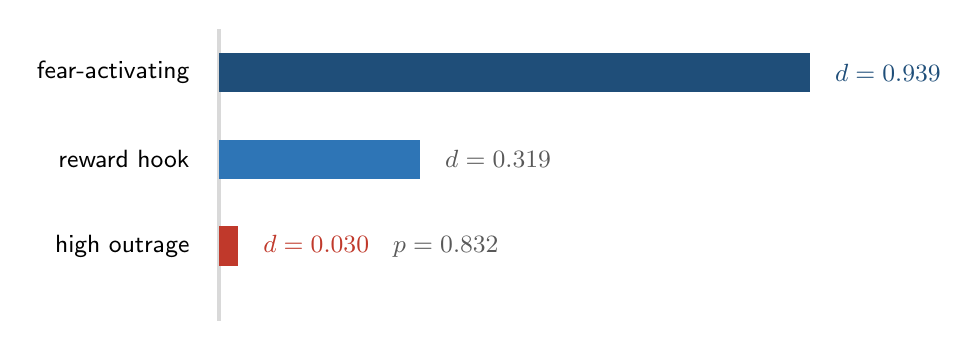
\begin{tikzpicture}[font=\small]
  \draw[mist,line width=1.2pt] (0,-0.55) -- (0,3.15);
  \node[left] at (-0.25,2.6) {fear-activating};
  \fill[navy] (0,2.35) rectangle (7.51,2.85);
  \node[right,navy] at (7.7,2.6) {\textbf{$d = 0.939$}};

  \node[left] at (-0.25,1.5) {reward hook};
  \fill[midblue] (0,1.25) rectangle (2.55,1.75);
  \node[right,slate] at (2.75,1.5) {$d = 0.319$};

  \node[left] at (-0.25,0.4) {high outrage};
  \fill[ember] (0,0.15) rectangle (0.24,0.65);
  \node[right,ember] at (0.44,0.4) {\textbf{$d = 0.030$} \; {\color{slate}$p = 0.832$}};
\end{tikzpicture}
\end{center}

\vspace{0.8em}
Cohen's $d$ against the neutral baseline. \alert{Outrage is the category the proposal expected
to separate most,} and on the index it does not. Taken apart, it raises both networks:
affective $d = +0.507$, deliberative $d = +0.491$. Fear raises one only.
\end{frame}

\begin{frame}{Category cannot be told apart from source dataset}
\vspace{0.3em}
\begin{center}
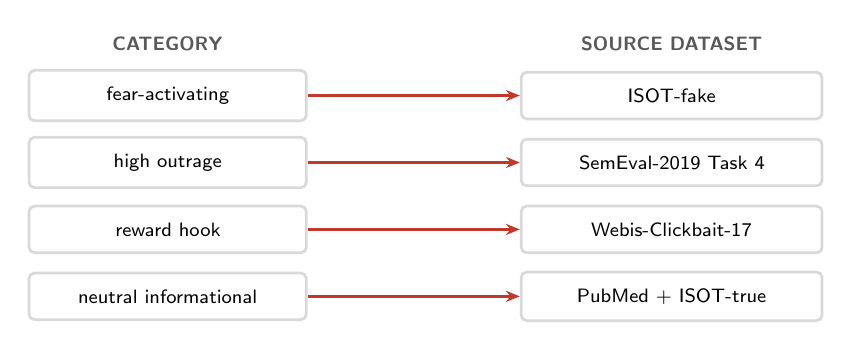
\begin{tikzpicture}[font=\scriptsize,
   c/.style={draw=mist,line width=1pt,rounded corners=2pt,fill=white,text width=3.1cm,
             align=center,inner sep=6pt},
   s/.style={draw=mist,line width=1pt,rounded corners=2pt,fill=white,text width=3.4cm,
             align=center,inner sep=6pt}]
  \node[c] (c1) at (0,2.55) {fear-activating};
  \node[c] (c2) at (0,1.70) {high outrage};
  \node[c] (c3) at (0,0.85) {reward hook};
  \node[c] (c4) at (0,0.00) {neutral informational};
  \node[s] (s1) at (6.4,2.55) {ISOT-fake};
  \node[s] (s2) at (6.4,1.70) {SemEval-2019 Task 4};
  \node[s] (s3) at (6.4,0.85) {Webis-Clickbait-17};
  \node[s] (s4) at (6.4,0.00) {PubMed + ISOT-true};
  \foreach \i in {1,2,3,4}
    \draw[-{Stealth[length=5pt,width=4pt]},line width=1.1pt,ember] (c\i) -- (s\i);
  \node[above,slate] at (0,3.0) {\textbf{CATEGORY}};
  \node[above,slate] at (6.4,3.0) {\textbf{SOURCE DATASET}};
\end{tikzpicture}
\end{center}

\vspace{0.7em}
One source per category, so the separation is between \emph{corpora} and cannot be attributed
to \emph{framing}. Length is controlled; provenance is not.
\end{frame}

\begin{frame}{A bag of words beats the index on the label, so the index is not a classifier}
\vspace{0.6em}
\begin{columns}[T]
\begin{column}{0.48\textwidth}
\begin{center}
{\color{slate}\fontsize{38}{38}\selectfont\bfseries 0.6274}\\[0.5em]
{\color{slate}AUC, the index, nothing fitted}
\end{center}
\end{column}
\begin{column}{0.48\textwidth}
\begin{center}
{\color{ember}\fontsize{38}{38}\selectfont\bfseries 0.9758}\\[0.5em]
{\color{slate}AUC, TF-IDF + logistic, 5-fold}
\end{center}
\end{column}
\end{columns}

\vspace{1.2em}
{\small Same 400 rows, same label. Sentiment (VADER) sits at chance, $0.5392$. The same
words guess the \emph{source} 66\% of the time against 25\% chance, so much of the lexical
win is provenance.}

\vspace{0.8em}
\alert{The index is a field observable for the physics, not a detector.}
\source{Hutto \& Gilbert (2014), VADER.}
\end{frame}

\begin{frame}{Group-level claims hold at this precision; per-item claims do not}
\vspace{0.6em}
\begin{columns}[T]
\begin{column}{0.48\textwidth}
\begin{center}
{\color{navy}\fontsize{38}{38}\selectfont\bfseries 0.8725}\\[0.5em]
{\color{slate}ICC between two GPU sessions}
\end{center}
\vspace{0.8em}
{\small The separation replicates: $\eta^2 = 0.0888$ against $0.1068$.}
\end{column}
\begin{column}{0.48\textwidth}
\begin{center}
{\color{ember}\fontsize{38}{38}\selectfont\bfseries 12.8\%}\\[0.5em]
{\color{slate}of items reverse direction}
\end{center}
\vspace{0.8em}
{\small 51 of 400. Noise alone predicts 55, so no verdict on one article is ever made.}
\end{column}
\end{columns}
\end{frame}

\begin{frame}{The encoder returns a full cortical map, not a summary statistic}
\vspace{-0.4em}
\begin{center}
\includegraphics[width=0.70\textwidth,trim=0 0 0 20,clip]{B3_per_vertex_fear_activating-0000.pdf}
\end{center}
\vspace{-0.5em}
\begin{center}
{\color{slate}\small One fear-activating item at all 20,484 vertices, painted above the map's
70th percentile. Nothing is smoothed, interpolated or simulated.}
\end{center}
\end{frame}

% ================================================================ ACT IV
\section{The physics}
\act{04}{The physics}{What a measured field is worth.}

\begin{frame}{Media enters the mean-field model as a field on the measured observable}
\vspace{0.7em}
Each person holds an opinion $\pm 1$, is pulled toward neighbours by $J$, and pushed by media
with field $h = \alpha X$, where $X$ is the measured observable:
\[
m = \tanh(\beta J m + h)
\]
\[
F(m) = a m^2 + b m^4 - hm, \qquad a = \frac{1-\beta J}{2}, \qquad b = \frac{1}{12}
\]

\vspace{0.4em}
{\color{slate} Coefficients derived, not assumed; this corrects the proposal's $a$ and $b$.
The solver recovers the mean-field exponents.}
\end{frame}

\begin{frame}{The corpus does not identify the coupling, so no value is quoted}
\vspace{1.2em}
\textbf{Tried.} Fit the outcome to the measured index and read off $\alpha$.

\vspace{0.9em}
\textbf{Result.} Out of sample the fit does \emph{worse than the average}, and the estimate
depends on $\beta J$, which nothing here measures.

\vspace{0.9em}
\alert{So no value of $\alpha$ is quoted anywhere.}

\vspace{1.2em}
{\color{slate} What replaces it needs no fit at all: the bound on the next slide.}
\end{frame}

\begin{frame}{Any content observable must clear a bound to drive a transition}
\vspace{0.2em}
\begin{columns}[T]
\begin{column}{0.56\textwidth}

\includegraphics[width=\textwidth]{F6_alpha_required.pdf}
\end{column}
\begin{column}{0.40\textwidth}
\vspace{1.2em}
\begin{center}
{\fontsize{23}{27}\selectfont\color{navy}
$\alpha \;\ge\; \dfrac{h_c(\beta J)}{\Delta X}$}
\end{center}

\vspace{1.0em}
{\small What $\alpha$ \emph{would have to be} for media to tip opinion, for any observable,
before any data. Within the mean-field model.}

\vspace{1.0em}
{\small Measured $\Delta X = 0.1241$ gives \\ \alert{$\alpha \ge 4.29$ at $\beta J = 2$}.}
\end{column}
\end{columns}
\end{frame}

% ================================================================ ACT V
\section{Standing}
\act{05}{Standing}{What holds, and what is still open.}

\begin{frame}{Against real brains the encoder is weakly positive, not anti-correlated}
\vspace{0.4em}
A company audit says the checkpoint this project runs is \textbf{anti-correlated} with real
cortex. Tested here on public fMRI:

\vspace{0.8em}
\begin{center}
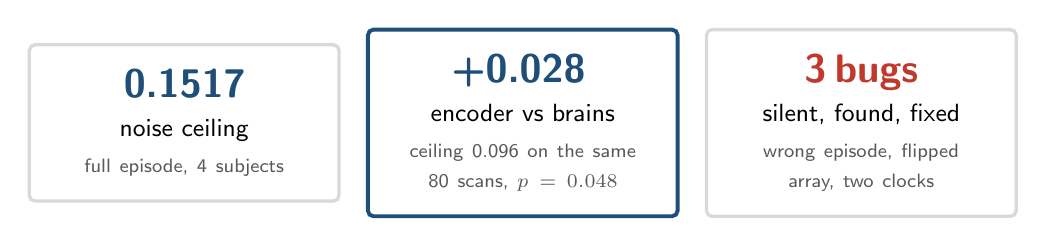
\begin{tikzpicture}[font=\small]
  \node[draw=mist,line width=1.2pt,rounded corners=2pt,fill=white,inner sep=9pt,
        text width=3.3cm,align=center] at (0,0)
       {{\color{navy}\bfseries\Large 0.1517}\\[0.35em] noise ceiling\\[0.2em]
        {\color{slate}\scriptsize full episode, 4 subjects}};
  \node[draw=navy,line width=1.4pt,rounded corners=2pt,fill=white,inner sep=9pt,
        text width=3.3cm,align=center] at (4.3,0)
       {{\color{navy}\bfseries\Large +0.028}\\[0.35em] encoder vs brains\\[0.2em]
        {\color{slate}\scriptsize ceiling 0.096 on the same 80 scans, $p = 0.048$}};
  \node[draw=mist,line width=1.2pt,rounded corners=2pt,fill=white,inner sep=9pt,
        text width=3.3cm,align=center] at (8.6,0)
       {{\color{ember}\bfseries\Large 3 bugs}\\[0.35em] silent, found, fixed\\[0.2em]
        {\color{slate}\scriptsize wrong episode, flipped array, two clocks}};
\end{tikzpicture}
\end{center}

\vspace{0.8em}
Positive, weak, and not yet decisive on two minutes of film.
\source{Algonauts 2025; Schaefer et al.\ (2018); audit: The Sapient Company (2026).}
\end{frame}

\begin{frame}{Four claims the work supports, and four it does not}
\vspace{0.7em}
\begin{columns}[T]
\begin{column}{0.47\textwidth}
{\color{navy}\bfseries SUPPORTED}
\vspace{0.8em}

{\small
$\bullet$\; A content observable that can be measured, with its reliability stated.

\vspace{0.6em}
$\bullet$\; That it separates these four corpora at $\eta^2 = 0.1068$, power attached.

\vspace{0.6em}
$\bullet$\; A bound any candidate observable must satisfy, usable before data exists.

\vspace{0.6em}
$\bullet$\; A noise ceiling on public fMRI, and a first check of the encoder against it.
}
\end{column}
\begin{column}{0.47\textwidth}
{\color{ember}\bfseries NOT SUPPORTED}
\vspace{0.8em}

{\small
$\bullet$\; That the index detects manipulation. Source is confounded; TF-IDF scores $0.9758$.

\vspace{0.6em}
$\bullet$\; Anything about the amygdala. The checkpoint does not predict it.

\vspace{0.6em}
$\bullet$\; Any value of the coupling $\alpha$. The corpus does not identify it.

\vspace{0.6em}
$\bullet$\; Any verdict on one article. 12.8\% reverse between sessions.
}
\end{column}
\end{columns}
\end{frame}

\begin{frame}{The work yields a dissertation and three papers}
\vspace{0.8em}
\begin{columns}[T]
\begin{column}{0.235\textwidth}
{\color{midblue}\bfseries 81 pp}\\[0.3em]
\textbf{Dissertation}\\[0.4em]
{\color{slate}\scriptsize Complete, review answered.}
\end{column}
\begin{column}{0.235\textwidth}
{\color{midblue}\bfseries 12 pp}\\[0.3em]
\textbf{Paper 1}\\[0.4em]
{\color{slate}\scriptsize The bound and the screening criterion. \emph{Physica A}.
Independent of the scan.}
\end{column}
\begin{column}{0.235\textwidth}
{\color{midblue}\bfseries 16 pp}\\[0.3em]
\textbf{Paper 2}\\[0.4em]
{\color{slate}\scriptsize The instrument, the corpus, the field bound. \emph{Physica A}.}
\end{column}
\begin{column}{0.235\textwidth}
{\color{midblue}\bfseries 8 pp}\\[0.3em]
\textbf{Paper 3}\\[0.4em]
{\color{slate}\scriptsize The noise ceiling and a check of the encoder against real brains.
\emph{Imaging Neuroscience}.}
\end{column}
\end{columns}

\vspace{1.4em}
{\color{mist}\hrule height 1.2pt}
\vspace{0.9em}

Every number in all four comes from a re-runnable script. Nothing is transcribed by hand.
\end{frame}

% ================================================================ CONCLUSIONS
\begin{frame}{Conclusions}
\vspace{0.6em}
\begin{enumerate}
\item \textbf{A field observable can be measured from content.} The instrument runs, the
corpus is complete, and reliability is measured rather than assumed: ICC $= 0.8725$.

\vspace{0.45em}
\item \textbf{It separates four corpora at $\eta^2 = 0.1068$, and the separation is
confounded with source.} Both halves are reported, the confound first.

\vspace{0.45em}
\item \textbf{The coupling is unidentified, so the thesis reports a bound instead.} With
$\Delta X = 0.1241$, $\alpha \ge 4.294$ at $\beta J = 2$ --- a constraint on any future
proposal of this mechanism.

\vspace{0.45em}
\item \textbf{The encoder is weakly positive against real brains, not anti-correlated.}
$r = +0.028$ against a ceiling of $0.096$ on the same scans; not yet decisive.
\end{enumerate}

\vspace{1.0em}
{\color{mist}\hrule height 1.2pt}
\vspace{0.6em}
{\color{slate}\small Brian Mwai \;$\cdot$\; 1050555 \;$\cdot$\;
\texttt{monarch-4iy.pages.dev} \;$\cdot$\; \texttt{github.com/brn-mwai/monarch}}
\end{frame}

% ================================================================ REFERENCES
\begin{frame}{References}
\vspace{0.5em}
{\footnotesize
Ahmed, H., Traore, I., Saad, S. (2017). Detection of online fake news using n-gram analysis
and machine learning. \emph{ISDDC}.

\vspace{0.35em}
d'Ascoli, S. et al.\ (2025). TRIBE: a trimodal brain encoder for whole-brain fMRI response
prediction. Meta FAIR. arXiv:2507.22229.

\vspace{0.35em}
Gifford, A. T. et al.\ (2025). The Algonauts Project 2025 Challenge. arXiv:2501.00504.

\vspace{0.35em}
Glasser, M. F. et al.\ (2016). A multi-modal parcellation of human cerebral cortex.
\emph{Nature} 536, 171--178.

\vspace{0.35em}
Kiesel, J. et al.\ (2019). SemEval-2019 Task 4: hyperpartisan news detection.
\emph{SemEval}.

\vspace{0.35em}
Korbel, J., Dahdoul, R., Thurner, S. (2026). Empirical validation of the polarization
transition in a double-random field model of elections. \emph{Phys. Rev. Lett.} 136, 127402.

\vspace{0.35em}
Hutto, C. J., Gilbert, E. (2014). VADER: a parsimonious rule-based model for sentiment
analysis of social media text. \emph{ICWSM}.

\vspace{0.35em}
Potthast, M. et al.\ (2018). Crowdsourcing a large corpus of clickbait on Twitter.
\emph{COLING}, 1498--1507.

\vspace{0.35em}
The Sapient Company (2026). The Faceless Brain. Self-published technical report.

\vspace{0.35em}
Schaefer, A. et al.\ (2018). Local-global parcellation of the human cerebral cortex.
\emph{Cereb. Cortex} 28, 3095--3114.
}
\end{frame}

\end{document}
